\chapter{~Physical Quizzes~}

\section*{問1}
図1のように天井にくくりつけられたロープに人が片手でぶら下がり、静かに止まっています。\par
実はいま、ロープはまさに千切れる寸前の状態にあるのですがちぎれるとすればロープのどちら側が先に千切れるでしょうか。
\begin{description}
  \item[(A)] 左側の長い方
  \item[(B)] 右側の短い方
  \item[(C)] 確率は五分五分
\end{description}
\begin{figure}[H]
  \centering
  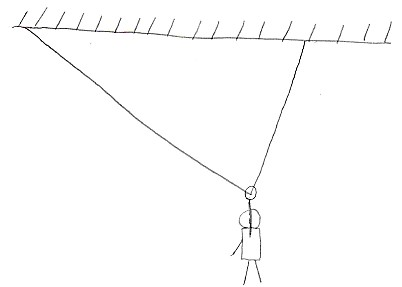
\includegraphics[height=4cm,clip]{nishimura/image/toi1.jpg}
  \caption{問1}
  \label{fig:toi1}
\end{figure}

\newpage
\section*{問2}
3月21日ころが春分の日、9月23日ころが秋分の日で\\
春分の日から秋分の日まで(春→夏→秋)は約186日\\
秋分の日から春分の日まで(秋→冬→春)は約179日\\
あります。さてこの約七日間の差はなぜ生じるのでしょうか。

\begin{description}
  \item[(A)] 歳差運動があるから冬季は一日が短いから
  \item[(B)] 冬季は一日が短いから
  \item[(C)] 太陽に近いとき、地球が速く動くから
  \item[(D)] 特に理由がない
\end{description}
※ヒント\ ケプラーの法則

\vspace{3zw}
\begin{figure}[H]
  \centering
  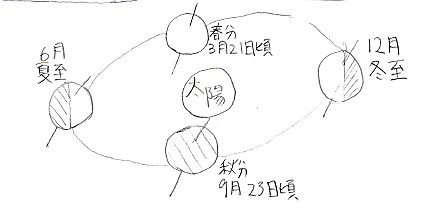
\includegraphics[height=6cm,clip]{nishimura/image/toi2.jpg}
  \caption{問2}
  \label{fig:toi2}
\end{figure}

\newpage
\section*{問3}
通常これらのうちで電磁波を放射しないのはどれでしょう。

\begin{description}
  \item[(A)] 太陽
  \item[(B)] 火山灰
  \item[(C)] 石炭
  \item[(D)] この本に使われている紙
  \item[(E)] どれも電磁波を放射している
\end{description}
※ヒント\ ウィーンの変位則
\vspace{3zw}
\begin{figure}[H]
  \centering
  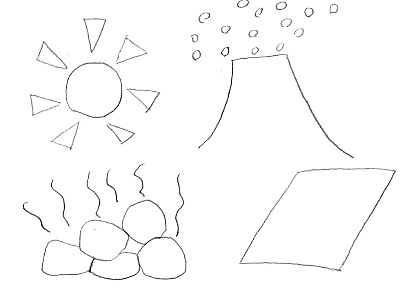
\includegraphics[height=7cm,clip]{nishimura/image/toi3.jpg}
  \caption{問3}
  \label{fig:toi3}
\end{figure}

\newpage
\section*{解答}
\section*{問1}
 解答 (B) \par
人は静かに止まっているので、人に働く外力はつりあっています。(外力は人の重力と重力の逆向きで大きさの等しい上向きの力)
ここで上向きの力はロープの左右両側の張力を合成したものです。よって下図のようになります。下図より右のロープのほうが左のロープより大きな張力が働くので右側が先に千切れます。
\begin{figure}[H]
  \centering
  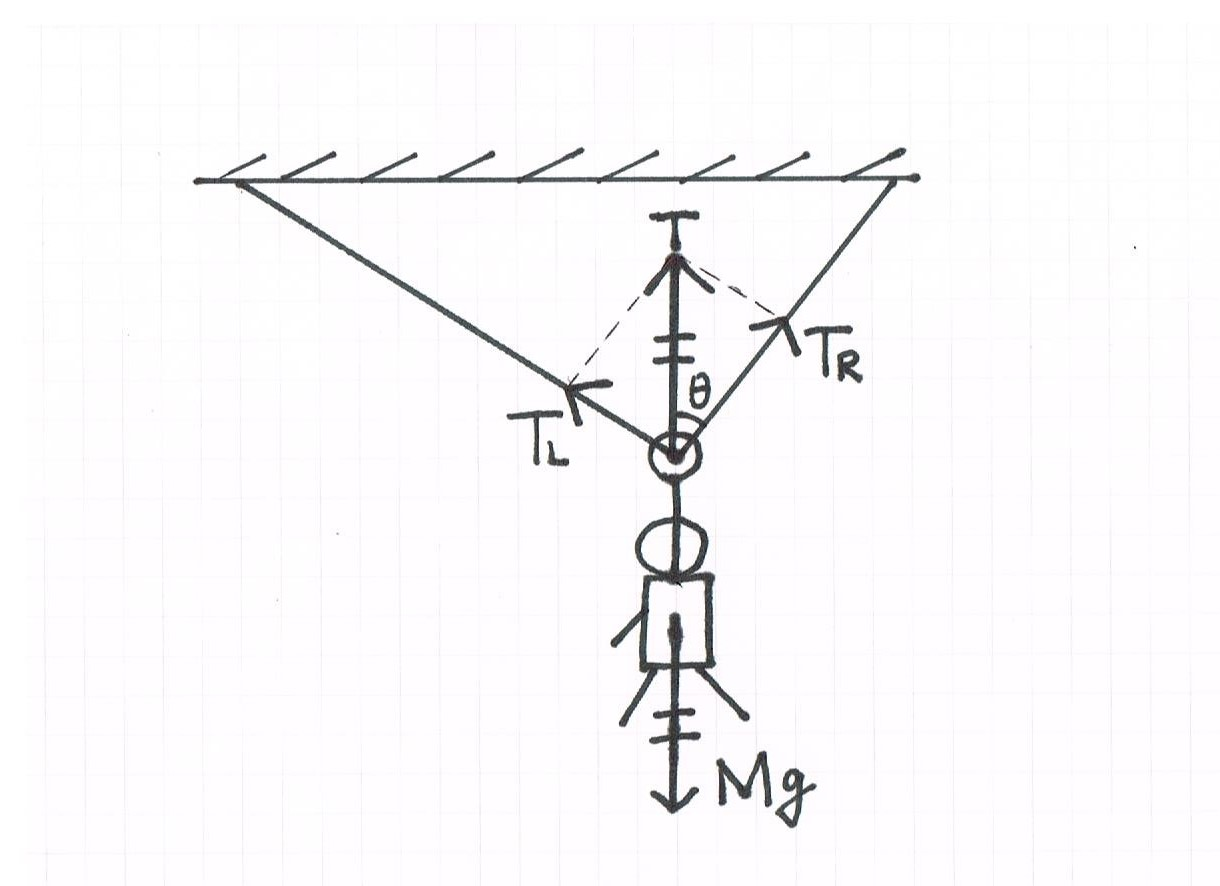
\includegraphics[height=4cm,clip]{nishimura/image/toi1_A.jpg}
  \caption{問3}
  \label{fig:toi3}
\end{figure}
この現象を数式を使って説明すると、
 人間の質量をM[kg]、重力加速度をg[$m/s^2$]とする。右側の糸に働く張力を$ T_R$[N]、左側の糸に働く張力を$T_L$[N]、二つの張力の合力をT[N]とすると、図より次の3式が得られる。
\begin{eqnarray*}
T&=&Mg\\
T_R&=&T \cos \theta\\
T_L&=&T \sin \theta\\
\end{eqnarray*}

ここで$\theta<45$度より\\
$$T \cos \theta >T \sin \theta \longrightarrow   T_R > T_L$$ \par
したがって糸が千切れるとすれば右側が切れる。

\newpage
\section*{問2}
 解答 (C) \par
ケプラーの法則
\begin{enumerate}
\item	太陽系の惑星は太陽を一つの焦点とした楕円軌道を公転する(第一法則)
\item	太陽と惑星とを結ぶ積分が単位時間に描く面積は一定である(第二法則)
\item	惑星の軌道の超半径の三乗と惑星の公転周期の二乗の比は、どの惑星に於いても一定である(第三法則)
\end{enumerate}\par
1より地球と太陽の距離は変化します。②より地球と太陽の距離が近いほど公転軌道を早く移動します。そして現在は北半球が冬の時その距離が小さくなるので冬至のころに最も移動速度が大きくなります。よって秋分→冬至→春分までの日数のほうが春分→夏至→秋分までの日数よりも短くなります。

% \newpage
\section*{問3}
 解答 (E) \par
ウィーンの変位則
物体から放射される光のうちエネルギー密度が最大になる光の波長$\lambda$は物体の本土に反比例して短くなる
\[
\lambda = \frac{k}{T}
\]
ここで$k$は比例定数、$T$は温度

すべての物質はエネルギーを電磁波として放射しています。最も多くのエネルギーを放射する電磁波の周波数を$f$とすれば、$f$と$T$には比例関係があります。この紙も例外ではなく、低温のため低周波数ではありますが、電磁波を放射しています。

\newpage
\section*{参考\ ケプラーの三法則}
\begin{description}
\item[第1法則] 惑星は太陽を一つの焦点とする楕円軌道を描く。
\item[第2法則] 惑星が太陽のまわりに描く面積速度は,各惑星毎に一定である。
\item[第3法則] 惑星の公転周期$T$の2乗は,楕円の長軸の長さaの3乗に比例する。
\end{description}
\subsection*{ケプラーの第一法則について}
ケプラーの第一法則が発見されるまでは、惑星は太陽を中心に完全な円上を運動しているとされていた。もし、軌道が完全な円だとしたら図\ref{fig:kep1}のようになる。
\begin{figure}[H]
  \centering
  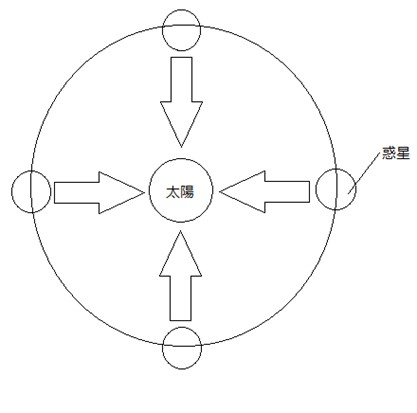
\includegraphics[height=5cm,clip]{nishimura/image/kep1.jpg}
  \caption{ケプラーの第一法則}
  \label{fig:kep1}
\end{figure}
この場合、惑星と太陽の距離はどこから測っても同じになる。
しかし、観測結果は惑星の位置によって太陽との距離が変化した。(図\ref{fig:kep1_1})\par
つまり、軌道は楕円軌道だった。
\begin{figure}[H]
  \centering
  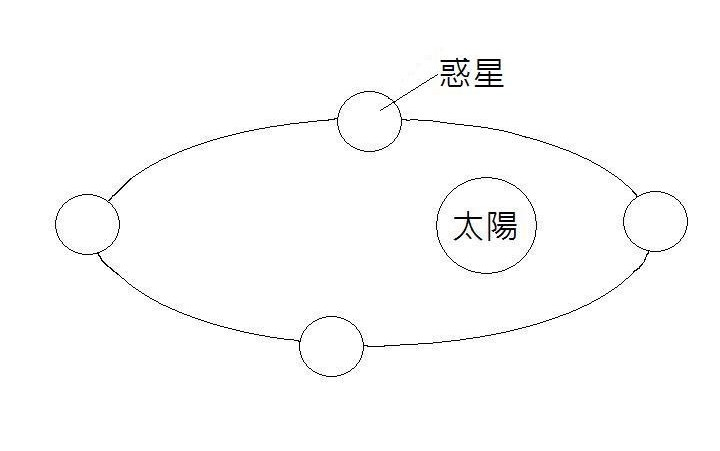
\includegraphics[height=4cm,clip]{nishimura/image/kep1_1.jpg}
  \caption{ケプラーの第一法則}
  \label{fig:kep1_1}
\end{figure}

\subsection*{ケプラーの第二法則について}
万有引力は中心に向かう力,中心力だから惑星の運動の角運動量Lは保存する。すなわち角運動量はその方向が惑星の軌道面に垂直な z 方向の成分しかなく,その大きさは極座標で表すと
\begin{eqnarray*}
L_z &=& m(xv_y-yv_x)\\
&=&mr\cos \theta \left(\frac{\rm{d}r}{\rm{d}t}\sin \theta + r\cos \theta \frac{\rm{d}\theta}{\rm{d}t}\right) - mr\sin \theta \left(\frac{\rm{d}r}{\rm{d}t}\cos \theta - r\sin \theta \frac{\rm{d}\theta}{\rm{d}t}\right) \\
&=& m r^2\frac{\rm{d}\theta}{\rm{d}t}
\end{eqnarray*}
となる。\par
したがって角運動量が一定は
\begin{eqnarray*}
L_z = m r^2\frac{\rm{d}\theta}{\rm{d}t} = D
\end{eqnarray*}
と書ける。\par
一方,面積速度は $\frac{1}{2}r^2 \frac{\rm{d}\theta}{\rm{d}t}     (=Aとする)$
であったので
\begin{eqnarray*}
\frac{1}{2}r^2 \frac{\rm{d}\theta}{\rm{d}t} = \frac{L_z}{2m} = \frac{D}{2m} = const
\end{eqnarray*}
となり,第 2 法則が導かれた。

\newpage
\subsection*{ケプラーの第三法則について}
惑星の楕円軌道の長軸 a と短軸 b はそれぞれ
\begin{eqnarray*}
\rm{a} &=&  \frac{\rm{b}^2}{a}\frac{\rm{a}^2}{\rm{b}^2} = \frac{l}{1-\epsilon ^2}\\
\rm{b} &=& \frac{\rm{b}^2}{a}\frac{\rm{a}}{\rm{b}} = \frac{l}{\sqrt{1-\epsilon ^2}}\\
\end{eqnarray*}
と表される。惑星の公転周期$T$は楕円の面積$S$を 面積速度$A$で割った時間であるから
\begin{eqnarray*}
  S = \pi \rm{ab} = \frac{\pi l^2}{(1-\epsilon ^2)^{3/2}}
\end{eqnarray*}
より
\begin{eqnarray*}
  T = \frac{S}{A} = \frac{\pi l^2}{A(1-\epsilon ^2)^{3/2}}
\end{eqnarray*}
この式の両辺を 2 乗すると
\begin{eqnarray*}
  T^2 = \frac{\pi^2 l}{A^2}\left( \frac{l}{1-\epsilon ^2}\right)^{3} = \frac{\pi^2 l \rm{a}^3}{A^2}
\end{eqnarray*}
となる。ゆえに
\begin{eqnarray*}
  \frac{T^2}{\rm{a}^3} = \frac{\pi^2}{A^2} = \frac{4\pi^2}{C}
\end{eqnarray*}
となり,ケプラーの第 3 法則が証明された。


\section*{参考文献}
\begin{enumerate}
  \item	ポール・G・ヒューイット作 松森靖夫 編著「傑作!物理パズル50」講談社 P.233
  \item	瀬戸悟「ケプラーの法則と万有引力」\\
  http://www.ishikawa-nct.ac.jp/lab/e/seto/www/files/kepler.pdf
  % HTTP://WWW.ISHIKAWA-NCT.AC.JP/LAB/E/SETO/WWW/FILES/KEPLER.PDF
\end{enumerate}
